\documentclass[a4paper,12pt]{extarticle}

\usepackage[T1]{fontenc}
\usepackage[utf8]{inputenc}

\usepackage[]{parskip}
\usepackage{hyperref, wrapfig, float, amsmath, adjustbox, array, pdflscape, soul, color, extsizes}

\renewcommand{\arraystretch}{2}
\renewcommand{\contentsname}{Spis treści}
\renewcommand{\refname}{Bibliografia}
\renewcommand{\figurename}{Rys.}

\usepackage{geometry}
\geometry{
  a4paper,
  margin=20mm,
  bottom=30mm
}

\usepackage{graphicx}
\usepackage{caption}
\usepackage{subcaption}
\usepackage[font=small,labelfont=bf]{caption}
\graphicspath{ {./images/}{../images/} }

\newcommand{\mathcolorbox}[1]{
  \begin{center}
    \colorbox{yellow}{$\displaystyle #1$}
  \end{center}
}
\newcommand{\pvec}[1]{
  \vec{#1}\mkern2mu\vphantom{#1}
}
\newcommand{\angstrom}{\mbox{\normalfont\AA}}

\begin{document}
  \begin{titlepage}
    \begin{center}
      \vspace*{.05\textheight}
      \begin{figure}[H]
        \centering
        
\includegraphics[scale=.15]{logopp.png}
      \end{figure}
      \vspace*{.05\textheight}
      \huge\textbf{Politechnika Poznańska}\\
      \large\textbf{Wydział Inżynierii Materiałowej i Fizyki Technicznej}\\
      \large\textbf{Fizyka Techniczna}\\
      \vspace*{.05\textheight}
      \huge\textbf{Skaningowa mikroskopia tunelowa}\\
      \vspace*{.025\textheight}
      \large\textbf{Jakub Bąbelek}
    \end{center}
  \end{titlepage}

  \tableofcontents
  
  \clearpage
  \section{Wstęp}
  Niniejsza praca jest sprawozdaniem z laboratorium, odbytego w ramach przedmiotu
  Podstawy Nanotechnologii, mającego przybliżyć działanie mikroskopu STM

  \subsection{Historia STM}
  Pod koniec 1978 Gerd Binnig oraz Heinrich Rohrer, rozpoczęli badania właściwości
  bardzo cienkich warstw tlenków metali. Potrzebowali oni do tego urządzenia
  umożliwiającego im oglądanie powierzchni w skali atomowej. W roku 1982 skonstruowali
  oni pierwszy skaningowy mikroskop tunelowy.
  
  W 1986 zostali oni, za swój wynalazek, uhonorowani Nagrodą Nobla w dziedzinie fizyki.

  \subsection{Budowa i zasada działania STM}
  \begin{figure}[H]
    \centering
    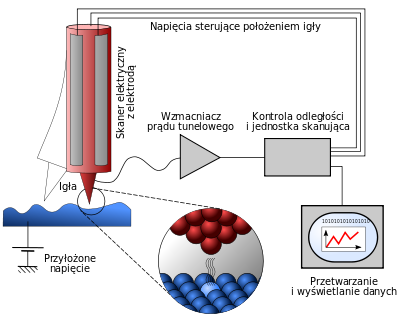
\includegraphics[scale=.75]{stmschematic.png}
    \caption{Schemat budowy STM}
    \label{fig:stmschem}
  \end{figure}
  
  Rysunek \ref{fig:stmschem} przedstawia schematyczną budowę mikroskopu skaningowego.
  W mikroskopie tym wykorzystuje się zjawisko tunelowe. Po zbliżeniu ostrza do próbki
  elektrony tunelują z jednego do drugiego przewodnika poprzez izolator, mierząc
  wartość prądu tunelowego oraz odnosząc go do wartości prądu odniesienia
  steruje się pętlą sprzężenia zwrotnego. Dane uzyskane w czasie pomiaru po
  obróbce komputerowej pozwalają zilustrować powierzchnię badanej próbki.


  \subsection{Zjawisko tunelowe}
  Zjawisko tunelowe jest kwantowo mechanicznym zjawiskiem w którym cząstka przenika
  przez barierę potencjału. Tunelowanie kwantowe nie jest możliwe z punktu widzenia
  mechaniki klasycznej, gdzie przeniknięcie takie wymaga aby cząstka posiadała
  energię potencjalną.
  Zjawisko to przewidziano i opisano teoretycznie juz w 1928 roku.

  \subsection{Tryby pracy}
  Skaningowy mikroskop tunelowy pracuje w dwóch trybach - stałej wysokości i prądu \ref{fig:stmmodes}.
  \begin{figure}[H]
    \centering
    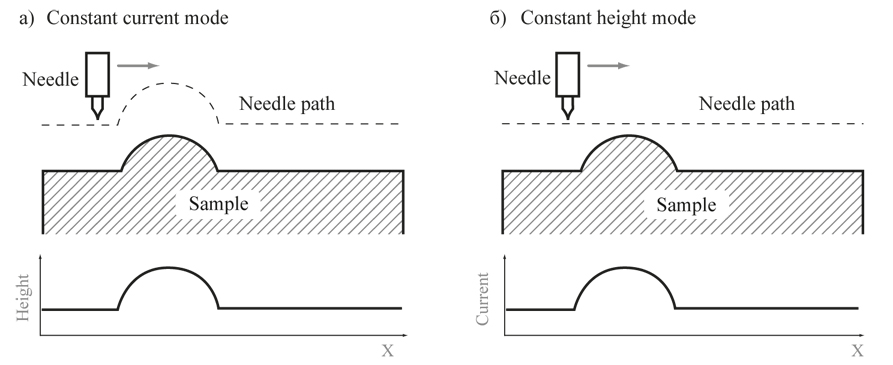
\includegraphics[scale=1.25]{stmmodes.jpg}
    \caption{Tryby pracy STM}
    \label{fig:stmmodes}
  \end{figure}

  \subsubsection{Tryb stałej wysokości}
  W trybie stałej odległosci, odległość pomiędzy badaną powierzchnią a igłą nie zmienia się.
  Informacje o topografii materiału otrzymuje się wówczas z wartości prądu.
  Wartość prądu tunelowego zmienia się wraz ze zmianami topografii powierzchni próbki.

  \subsubsection{Tryb stałego prądu}
  Tryb stałego prądu polega na utrzymaniu stałej wartości prądu tunelowego.
  Pozwala na to użycie pętli sprzężenia zwrotnego, która zapewnia utrzymanie
  stałej bariery potencjału. Cechą tego trybu jest duża dokładność odwzorowania powierzchni.

  \subsection{Odwrotne zjawisko piezoelektryczne}
  Odkryte przez braci Curie w 1880 roku odwrotne zjawisko piezoelektryczne polega
  na zmianie wymiaru materiału pod wpływem przyłożonego zewnętrznego pola
  elektrycznego. Zjawisko może dokonać zarówno odkształceń normalnych jak i tych
  związanych ze zmianą kształtu piezolementu.
  \begin{figure}[H]
    \centering
    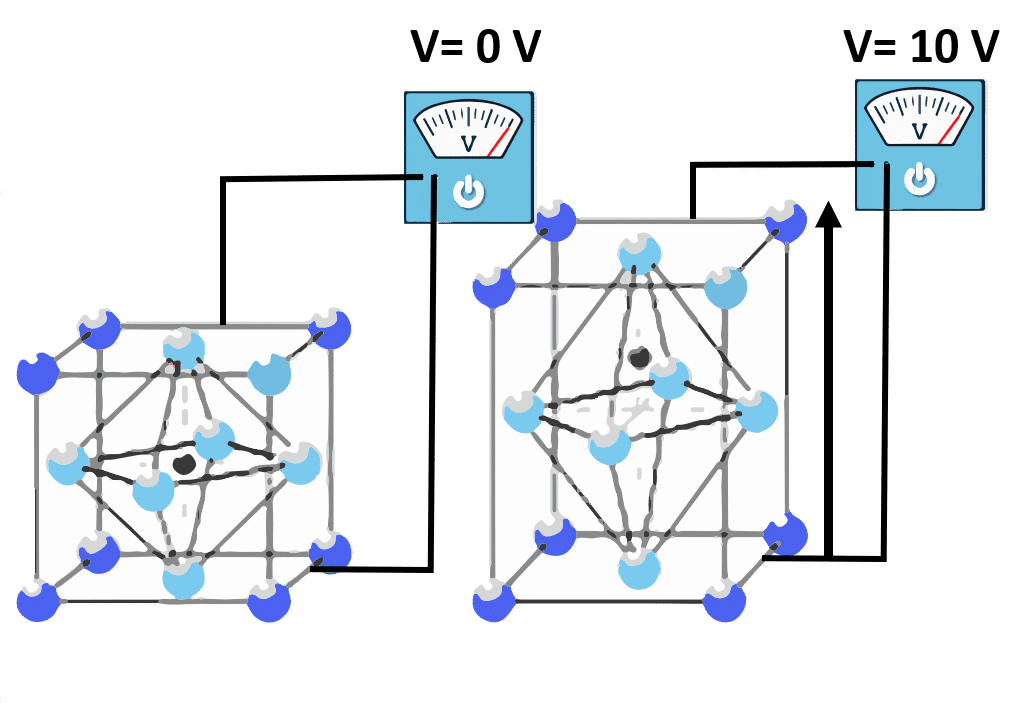
\includegraphics[scale=.5]{inversepiezoel.png}
    \caption{Odwrotne zjawisko piezoelektryczne}
    \label{fig:inversepiezoel}
  \end{figure}

  \subsection{Ostrze}
  Ostrze w skaningowym mikroskopach tunelowych wykonane jest najcześciej z
  platynowo-irydowego drutu o średnicy od 0,2 do 0,5mm. Idealny szpic zakończony
  jest jednym atomem - otrzymanie jednak takiego ostrza jest w praktyce bardzo trudne
  i za pomocą różnych metod próbuje się wykonać je możliwie jak najdokładniej.
  Najprostszą metodą jest ucięcie drutu pod kątem $45^o$ przy jednoczesnym jego "rozrywaniu".
  Innymi metodami jest m.in. elektrochemiczne trawienie w 30\% roztworze KOH czy
  ostrzenie na szlifierce szybkoobrotowej.

  \begin{figure}[H]
    \centering
    \begin{subfigure}{.5\textwidth}
      \centering
      \captionsetup{justification=centering}
      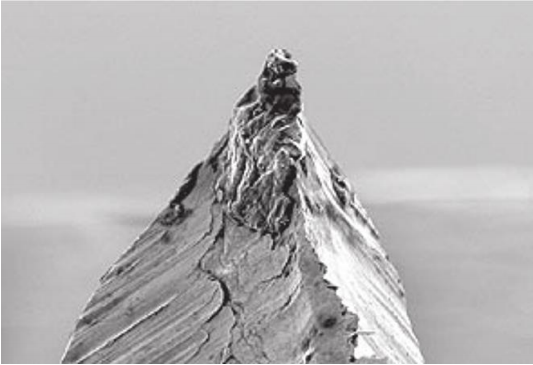
\includegraphics[scale=.5]{stmtip.png}
      \caption{Ostrze pod mikroskopem optycznym\\Źródło: www.nanosurf.com}
      \label{fig:stmtipmicro}
    \end{subfigure}%
    \begin{subfigure}{.5\textwidth}
      \centering
      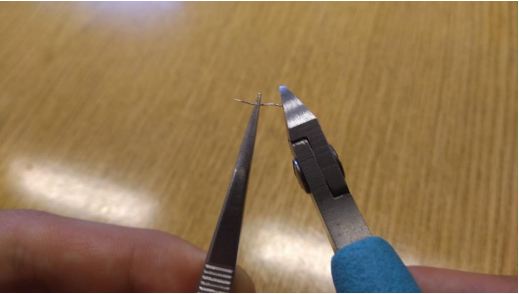
\includegraphics[scale=.6]{stmtipmaking.png}
      \caption{Preparowanie ostrza}
      \label{fig:stmtipmaking}
    \end{subfigure}
    \caption{Zdjęcia obrazujące ostrza}
    \label{fig:stmtip}
  \end{figure}

  \subsection{Próbka - HOPG}
  Highly Oriented Pyrolytic Graphite - Wysoce uporządkowana forma grafitu.
  Alotropowa odmiana węgla krystalizująca w płasko centrowanej sieci heksagonalnej.
  Charakteryzuje się wysokim przewodnictwem elektrycznym w kierunku równoległym
  do warstw. Jest odporny na wysoką temperaturę oraz bardzo kruchy.

  \begin{figure}[H]
    \centering
    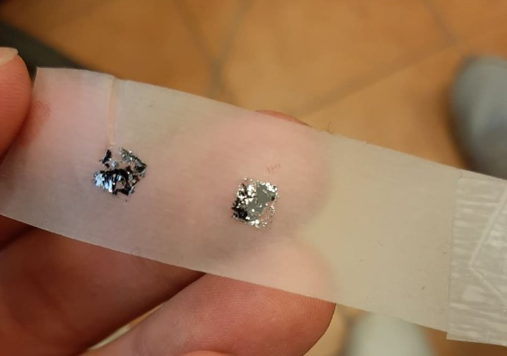
\includegraphics[scale=.75]{graphite.png}
    \caption{Warstwy grafitu ściagnięte z próbki przy pomocy taśmy}
    \label{fig:graphite}
  \end{figure}

  Aby przygotować próbkę do badania STM'em należy przy pomocy taśmy "scotch"
  oderwać wierzchnie warstwy grafenu pozbywając się z próbki nierównosci i
  utlenionych elementów materiału.

  \begin{figure}[H]
    \centering
    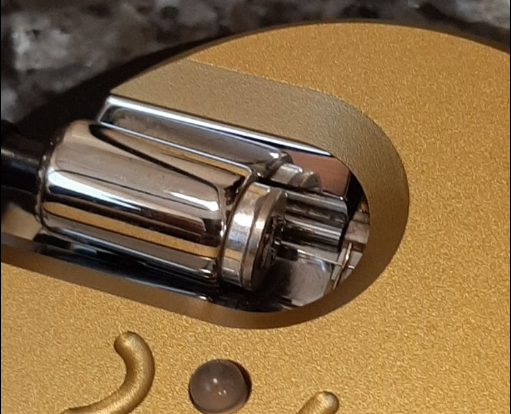
\includegraphics[scale=.75]{stmpomiar.png}
    \caption{Próbka grafitu umieszczona w mikroskopie}
    \label{fig:stmpomiar}
  \end{figure}

  \clearpage
  \section{Analiza pomiarów}
  W trakcie trwania laboratorium przeprowadziliśmy analizę próbki HOPG pod względem
  odległosci między atomami i uskoku na próbce grafitu.

  \subsection{Topografia}
  Rys. \ref{fig:data01} poddajemy obróbce w programie WSxM

  \begin{figure}[H]
    \centering
    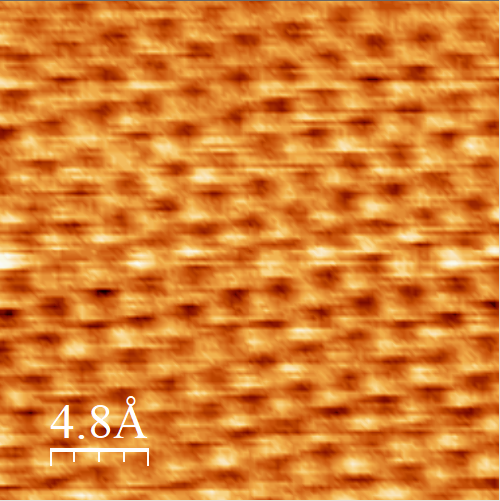
\includegraphics[scale=.5]{data01.png}
    \caption{Próbka grafitu przed obróbką w programie WSxM}
    \label{fig:data01}
  \end{figure}

  Stosujemy filtr "Flatten" (Rys. \ref{fig:data02}).
  \begin{figure}[H]
    \centering
    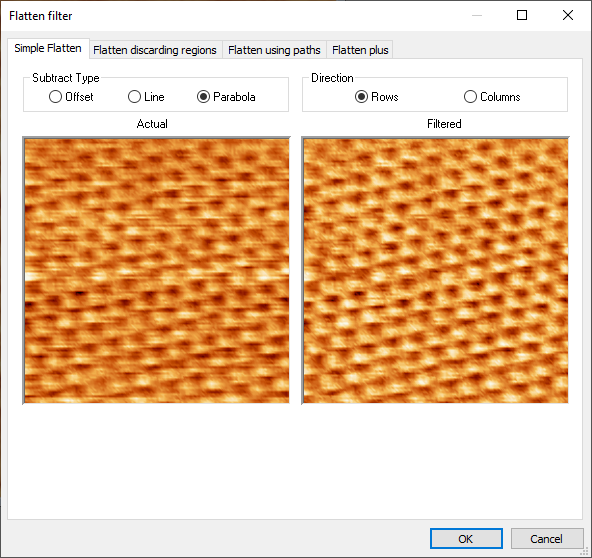
\includegraphics[scale=.5]{data02.png}
    \caption{Zrzut ekranu z programu WSxM}
    \label{fig:data02}
  \end{figure}
  \begin{figure}[H]
    \centering
    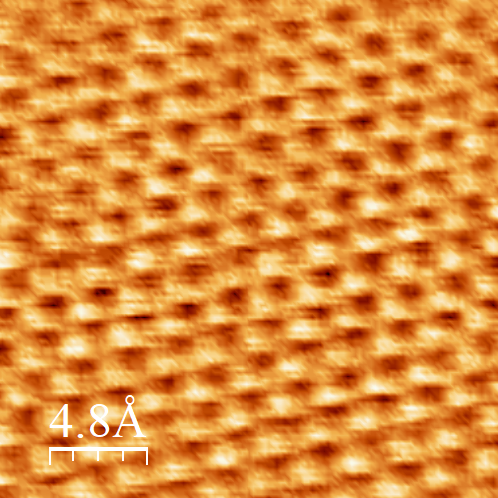
\includegraphics[scale=.5]{data03.png}
    \caption{Obraz po zastosowaniu filtra "Flatten"}
    \label{fig:data03}
  \end{figure}

  Używamy funkcji "Gaussian Smooth" z ustawieniami przedstawionymi na Rys. \ref{fig:data04}
  \begin{figure}[H]
    \centering
    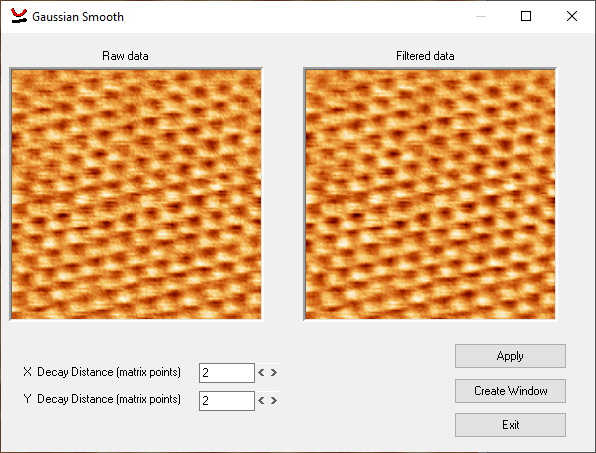
\includegraphics[scale=.5]{data04.png}
    \caption{Zrzut ekranu z programu WSxM}
    \label{fig:data04}
  \end{figure}
  \begin{figure}[H]
    \centering
    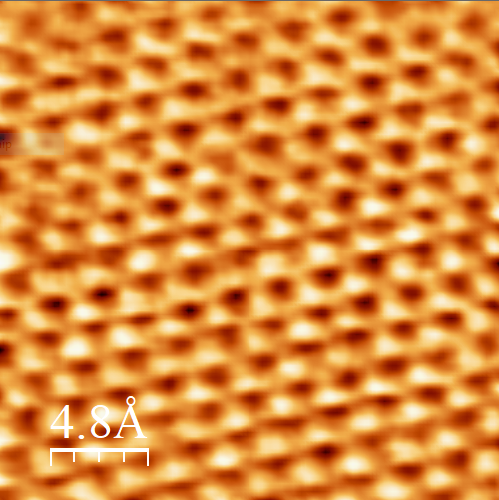
\includegraphics[scale=.5]{data05.png}
    \caption{Obraz po zastosowaniu "Gaussian Smooth"}
    \label{fig:data05}
  \end{figure}

  Wykonujemy transformatę Fouriera 2D - FFT
  \begin{figure}[H]
    \centering
    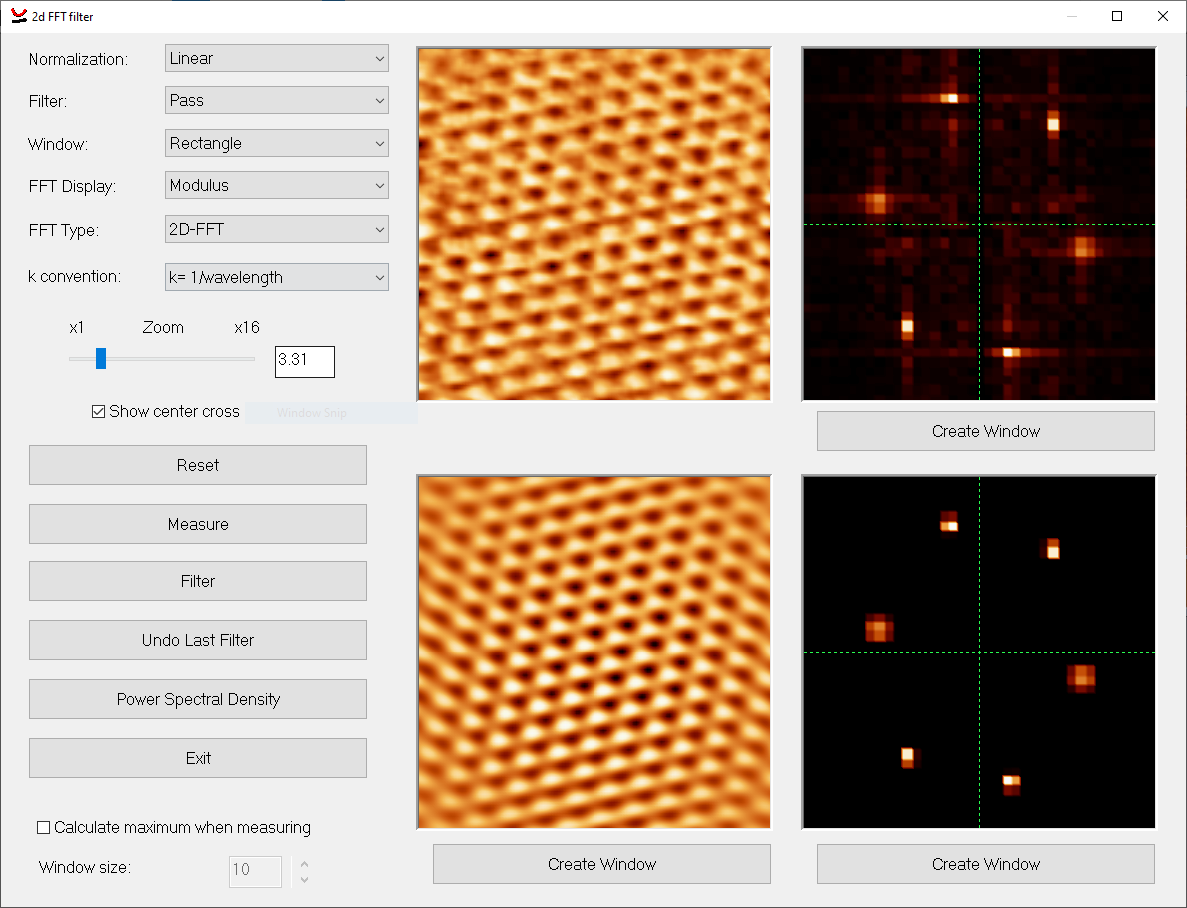
\includegraphics[scale=.5]{data06.png}
    \caption{Zrzut ekranu z programu WSxM}
    \label{fig:data06}
  \end{figure}
  \begin{figure}[H]
    \centering
    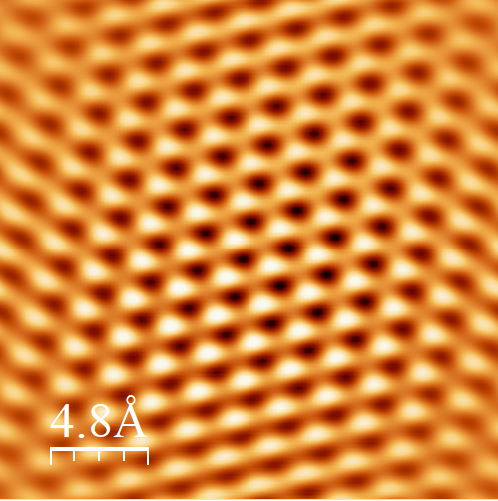
\includegraphics[scale=.5]{data07.png}
    \caption{Obraz po 2D - FFT}
    \label{fig:data07}
  \end{figure}

  Po powiększeniu najlepszego fragmentu badamy odległosci między atomami za pomocą
  funkcji "Plot Profile" oraz "Measure Distances" (Rys. \ref{fig:data08}) które zostaną przedstawione w
  następnym rozdziale.
  \begin{figure}[H]
    \centering
    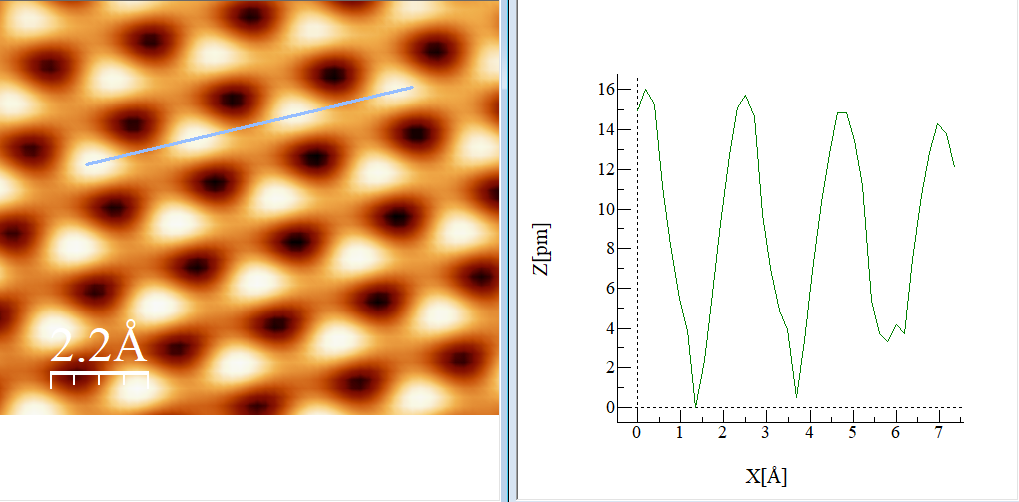
\includegraphics[scale=.5]{data08.png}
    \caption{Obraz z funkcji Plot Profile}
    \label{fig:data08}
  \end{figure}

  Po obróbce możemy przedstawić dane w postaci trójwymiarowej Rys. \ref{fig:data3dtopo}.
  Ze względu na atomową rozdzielczość STM, widoczne "wzniesienia" to pojedyczne
  atomy a właściwie rozkład gęstości chmur elektronowych.
  \begin{figure}[H]
    \centering
    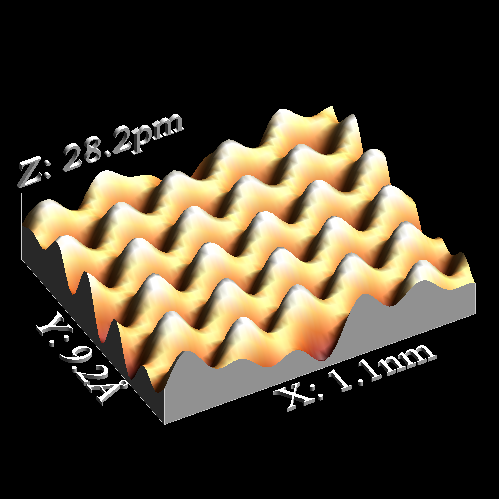
\includegraphics[scale=.5]{data3dtopo.png}
    \caption{Trójwymiarowe przedstawienie wcześniejszych obrazków}
    \label{fig:data3dtopo}
  \end{figure}

  \subsection{Uskok}
  Poza pomiarami w skali atomowej można też badać większe cechy powierzchni grafitu
  jak np. uskoki pomiędzy poszczególnymi warstwami.
  \begin{figure}[H]
    \centering
    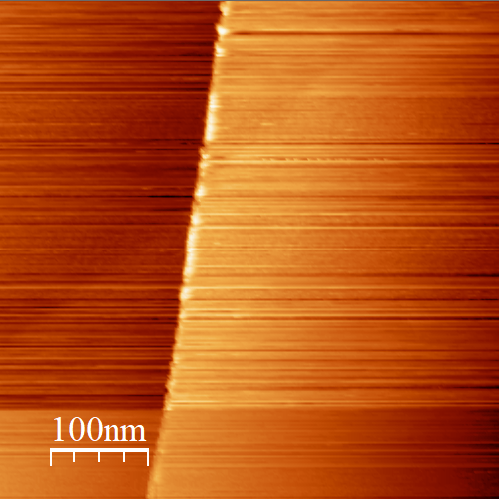
\includegraphics[scale=.5]{datauskok.png}
    \caption{Obraz 2D uskoku}
    \label{fig:datauskok}
  \end{figure}
  \begin{figure}[H]
    \centering
    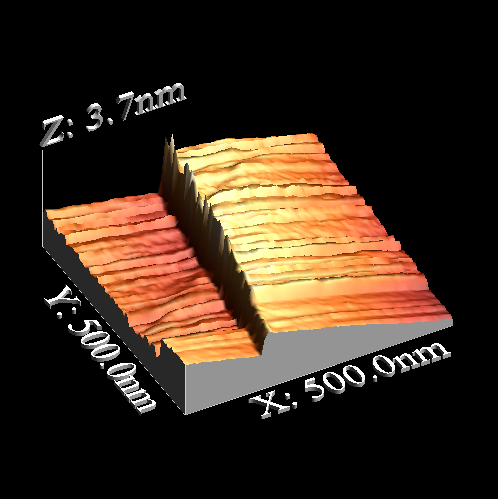
\includegraphics[scale=.5]{data3duskok.png}
    \caption{Trójwymiarowy obraz uskoku na próbce}
    \label{fig:data3duskok}
  \end{figure}
  \begin{figure}[H]
    \centering
    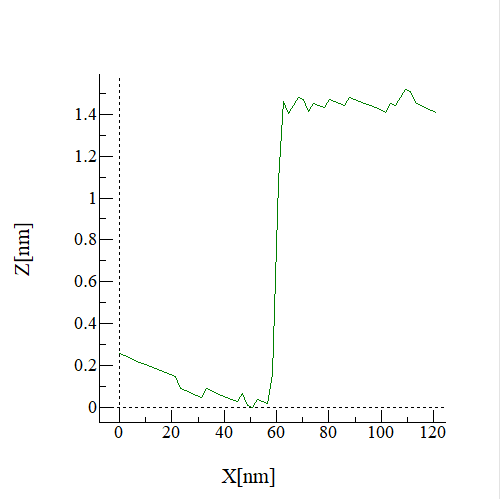
\includegraphics[scale=.5]{datauskokplot.png}
    \caption{Wykres wysokości w przekroju poprzecznym próbki}
    \label{fig:datauskokplot}
  \end{figure}

  \clearpage
  \section{Wyniki}
  Po obróbce danych należy obliczyć 

  \begin{table}[H]\centering
    \begin{adjustbox}{max width = \textwidth}
      \begin{tabular}{ccc|cc}
        \multicolumn{1}{c|}{\textbf{lp.}} & \multicolumn{1}{c|}{\textbf{Ilość atomów}} & \textbf{Długość [\r{A}]}  & \textbf{Odległość pomiędzy atomami [\r{A}]} &       \\ \hline
        \multicolumn{1}{c|}{1}            & \multicolumn{1}{c|}{3}                     & 6,749             & 2,250                               &       \\
        \multicolumn{1}{c|}{2}            & \multicolumn{1}{c|}{3}                     & 6,794             & 2,265                               &       \\
        \multicolumn{1}{c|}{3}            & \multicolumn{1}{c|}{4}                     & 8,660             & 2,165                               &       \\
        \multicolumn{1}{c|}{4}            & \multicolumn{1}{c|}{4}                     & 9,281             & 2,320                               &       \\
        \multicolumn{1}{c|}{5}            & \multicolumn{1}{c|}{4}                     & 8,884             & 2,221                               &       \\
        \multicolumn{1}{c|}{6}            & \multicolumn{1}{c|}{3}                     & 6,832             & 2,277                               &       \\
        \multicolumn{1}{c|}{7}            & \multicolumn{1}{c|}{4}                     & 8,882             & 2,221                               &       \\
        \multicolumn{1}{c|}{8}            & \multicolumn{1}{c|}{2}                     & 4,468             & 2,234                               &       \\ \hline
                                          &                                            & \textbf{Średnia [\r{A}]:} & 2,244 $\pm0,034$
        \end{tabular}
    \end{adjustbox}
  \end{table}

  Otrzymana z pomiarów wartość długości stałej sieci wynosi:
  \[ a = (2,244\pm0,034)\angstrom \]

  Wartość otrzymana różni się niewiele od wartości rzeczywistej, może byc to spowodowane
  zakłóceniami podczas przeprowadzania doświadczenia (wysoka czułość mikroskopu),
  niedokładnością w wykonywaniu analizy danych czy złą kalibracją urządzenia.
  
  \subsection{Charakterystyka prądowo-napięciowa}
  Dane wyekstrachowane za pomocą programu WSxM wykorzystano do sporządzenia
  uśrednionej krzywej I(V). Rys. \ref{fig:vicurve} przedstawia charakterystykę
  po wygładzeniu wykresu tak by zminimalizować wpływ szumów. Potwierdza on, że
  grafit to półprzewodnik o zerowej przerwie energetycznej.
  \begin{figure}[H]
    \centering
    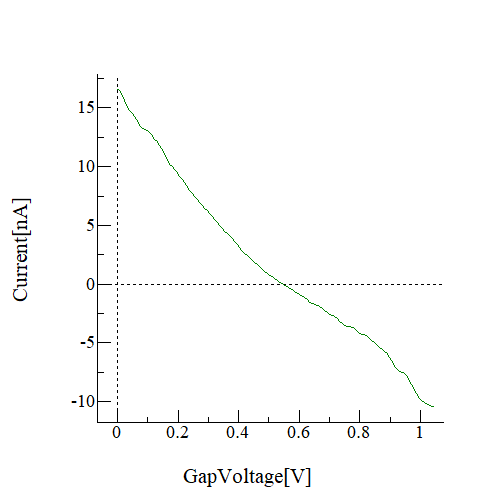
\includegraphics[scale=1]{vicurve.png}
    \caption{Charakterystyka I(V)}
    \label{fig:vicurve}
  \end{figure}

  \clearpage
  \begin{thebibliography}{9}
    \addcontentsline{toc}{section}{Bibliografia}
        
    \bibitem{binnig}
    Binnig, G.; Rohrer, H. (1986).
    \textit{Scanning tunneling microscopy}\\
    IBM Journal of Research and Development. 30 (4): 355–69.

    \bibitem{nobel}
    \textit{Press release for the 1986 Nobel Prize in physics}\\
    https://www.nobelprize.org/prizes/physics/1986/press-release/
  
    \bibitem{wsxm} 
    I. Horcas, R. Fernandez, J.M. Gomez-Rodriguez, J. Colchero, J. Gomez-Herrero and A. M. Baro, Rev. Sci. Instrum. 78, 013705 (2007)

  \end{thebibliography}

\end{document}